\documentclass[dvipdfmx,11pt]{kuisthesis}
%\documentclass[english]{kuisthesis} % 英語
\usepackage{graphicx}
\usepackage{tcolorbox}
\usepackage{caption}  % captionパッケージのインポート

\captionsetup{labelformat=empty}
\jtitle[画像処理と次数制約付き最小全域木に基づく細胞系統擬似時間の予測手法の改良]%	% 和文題目（内容梗概／目次用）
	{画像処理と次数制約付き最小全域木に基づく細胞系統擬似時間の予測手法の改良}	% 和文題目
\etitle{Improved method for predicting cell lineage pseudo-time based on image processing and constrained minimum spanning treee
}	% 英文題目
\jauthor{岩城　拓磨}				% 和文著者名
\eauthor{Iwaki Takuma}			% 英文著者名
\supervisor{阿久津　達也 教授}			% 指導教員名
\date{2025年2月6日}				% 提出年月日


\begin{document}
\maketitle					% 「とびら」の出力

\begin{jabstract}				% 和文梗概
  single-cell RNA-seq は、細胞のスナップショットを取得する技術であり、データ解析を通じて生物学的プロセスにおける変化の連続性を再構築することが可能である。
  細胞系統擬似時間解析のためのツールとして Slingshot や Monocle が広く利用されており、これらは最小全域木を用いて生物学的プロセスの軌道を予測している。しかし、これらのツールは「細胞の状態が一度に3つ以上には遷移しない」という生物学的前提を考慮していない。
  本研究では、Slingshot に対してこの課題を解決するための改良を加えた。本改良では、画像処理技術を用いて解析パラメータ（クラスタ数）を自動選択し、最小全域木に分岐制約を導入することで、生物学的に解釈しやすい解析を可能とした。この改良の有効性は、Bone marrow mononuclear cell、Hematopoiesis、Human fetal immune、および C. elegans データセットなどの公開データを用いて実証した。
\end{jabstract}

\begin{eabstract}				% 英文梗概
  Single-cell RNA sequencing (scRNA-seq) provides snapshots of individual cells, enabling the reconstruction of sequential changes in biological processes through data analysis. Various tools exist for pseudo-time analysis of cell lineage in biological processes, including Slingshot and Monocle, which utilize minimum spanning trees to predict trajectories. However, these tools do not account for the biological assumption that cellular states transition no more than three ways simultaneously.

  In this study, we present an improved version of Slingshot that addresses this limitation. Our enhancement employs image processing techniques to automatically select analysis parameters and introduces constraints on the minimum spanning tree to ensure biologically interpretable results. The effectiveness of this improvement was validated using publicly available datasets, including those from Bone marrow mononuclear cells, Hematopoiesis, Human fetal immune cells, and C. elegans.
\end{eabstract}

\tableofcontents				% 目次の出力

\section{はじめに}\label{sec-intro}		% 導入
細胞内での遺伝子発現の動的制御を理解するには、細胞分化や細胞周期などの時間依存的なプロセスを研究することが重要である。しかし、これらのプロセスにおいて、変化の正確な順序は一般に不明であり、指標となる遺伝子もほとんど特定されていない。また、細胞ごとに変化の速度が異なるため、各細胞の変化進行状況を外部から正確に判断することは極めて困難である。
近年、single-cell RNA-seq 技術の進展により、プロセスの異なる瞬間を反映した個々の細胞のスナップショットを取得することが可能となり、細胞の遺伝子発現の連続的な変化を解析できるようになった。この技術では、既知のマーカー遺伝子や同期された細胞を前提とせず、細胞の内部状態に基づいてプロセス内での位置（細胞擬似時間）を推定することが可能である。
single-cell RNA-seq データを用いた細胞擬似時間推定手法の1つに Slingshot がある。Slingshot は、クラスタリングされたデータを用い、最小全域木と同時主曲線アルゴリズムを組み合わせて滑らかな曲線を描画するツールである。このツールは他の解析ツールと併用しやすく設計されており、生物学的プロセスを通過する細胞に関する知見を明らかにするために広く利用されている。
しかし、Slingshot には以下の課題が存在する。第一に、クラスタ数をユーザーが指定する必要があるが、この数は最小全域木の構築や曲線の結果に大きく影響するにもかかわらず、有効な決定方法が提示されていない。第二に、「細胞の状態は一度に3つ以上に分岐しない」という生物学的前提が考慮されておらず、計算された曲線が3つ以上に分岐する可能性がある。
本研究では、細胞の内部状態データを画像として認識し、細線化アルゴリズムを活用してクラスタ数を自動的に決定する手法を提案する。また、最小全域木の構築時に分岐制約を導入し、細胞状態が3つ以上に分岐しないよう改良することで、生物学的に解釈しやすい細胞擬似時間の計算を実現した。

\section{結果}\label{sec-instruction}
\subsection{改良の概要}\label{subsec-instruction-1}
\bigskip
図1は、本改良が細胞の軌跡を推測するプロセスをまとめたものである。
おおまかに2次元データ全体の輪郭を細線化によって、おおまかな木構造を得ることができる。
その木構造の葉と分岐の数の合計をnとして、入力データをクラスタリングする。
クラスタリング済データを用いて制約を追加した最小全域木の構築する。
最小全域木と入力データを使用して、slingshotのフィッティングを行う。

まずumap等で2次元に次元削減したデータを入力として受け取る。
入力データのアルファシェイプの面積aを計算する。
図~\ref{fig-1}は、本研究で提案する改良が細胞の軌跡を推測するプロセスを示している。本改良は以下のステップで構成される。

\begin{enumerate}
    \item \textbf{細線化による木構造の抽出}  
    入力された2次元データ全体の輪郭を細線化アルゴリズムにより処理し、おおまかな木構造を取得する。この木構造は、データの大まかな分岐と形状を反映する。
    
    \item \textbf{クラスタ数の決定}  
    木構造から葉と分岐の数を抽出し、それらの合計を$n$としてクラスタ数を自動的に決定する。その後、入力データをこのクラスタ数に基づいてクラスタリングする。
    
    \item \textbf{制約付き最小全域木の構築}  
    クラスタリング済みデータを用いて、細胞状態が一度に3つ以上に分岐しないという生物学的制約を考慮した最小全域木を構築する。
    
    \item \textbf{Slingshotによるフィッティング}  
    制約付き最小全域木と入力データを基に、\texttt{Slingshot} を使用して滑らかな軌跡を描画する。これにより、生物学的に解釈しやすい細胞の擬似時間推定が可能となる。
\end{enumerate}

データの分散値を用いて初期の解像度bをきめ、bの10倍までのb刻みの解像度を用いて、入力データを画像に変換する。

\begin{tcolorbox}[colframe=black!70, colback=white, boxrule=0.2mm, width=\textwidth, arc=2mm]
  \label{fig-1}
  \begin{center}
      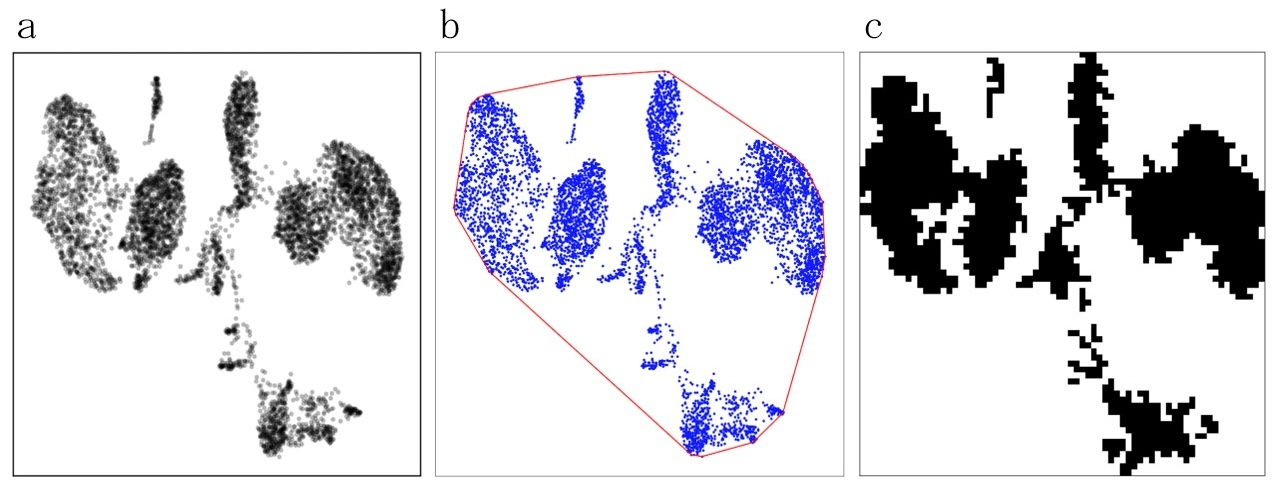
\includegraphics[width=\textwidth]{./img/Slide1.jpg}
      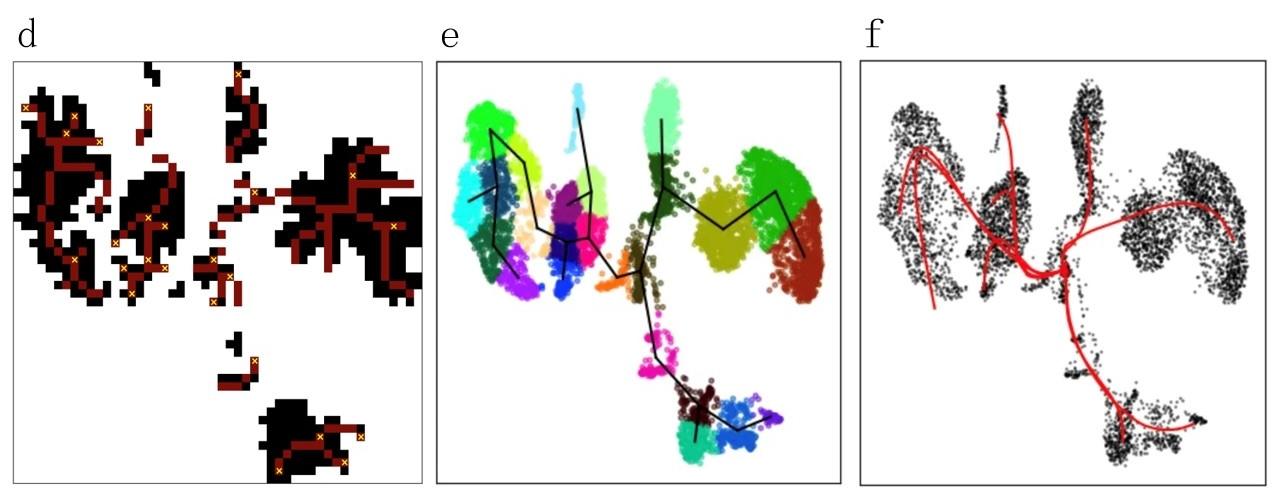
\includegraphics[width=\textwidth]{./img/Slide2.jpg}
  \end{center}
  \textbf{図１:} Bone marrow mononuclear cellを用いた改良後のslingshotによる解析結果
  \textbf{a} 入力データの散布図
  \textbf{b} 赤線が入力データのアルファシェイプ
  \textbf{c} 解像度を指定して画像化した入力データ
  \textbf{d} 赤線は細線化した結果。黄点の数をクラスタ数nとする。
  \textbf{e} クラスタ数nでクラスタリング済みデータに対して最小全域木を構築した結果
  \textbf{f} 最終的な解析結果
\end{tcolorbox}


\subsection{改良の効果}\label{subsec-instruction-2}
\begin{itemize}
  \item Bone marrow mononuclear cell
  ここに解析の方法や結果の解釈を書く
  \begin{tcolorbox}[colframe=black!70, colback=white, boxrule=0.2mm, width=\textwidth, arc=2mm]
    \begin{center}
        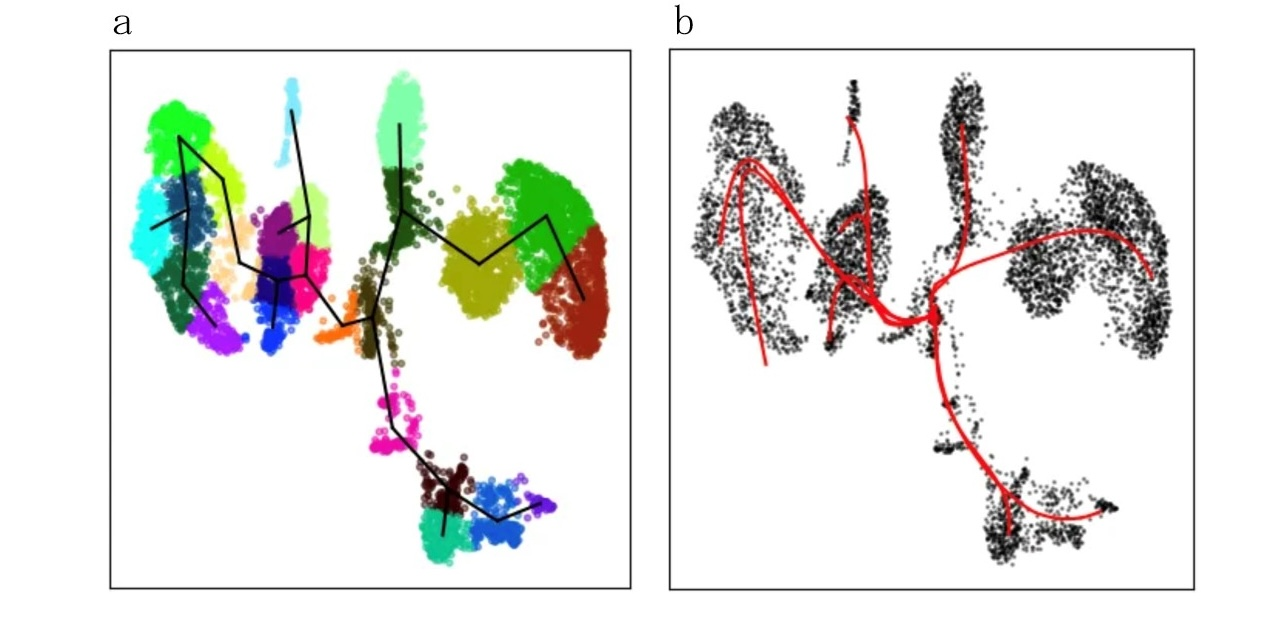
\includegraphics[width=\textwidth]{./img/Slide3.jpg}
        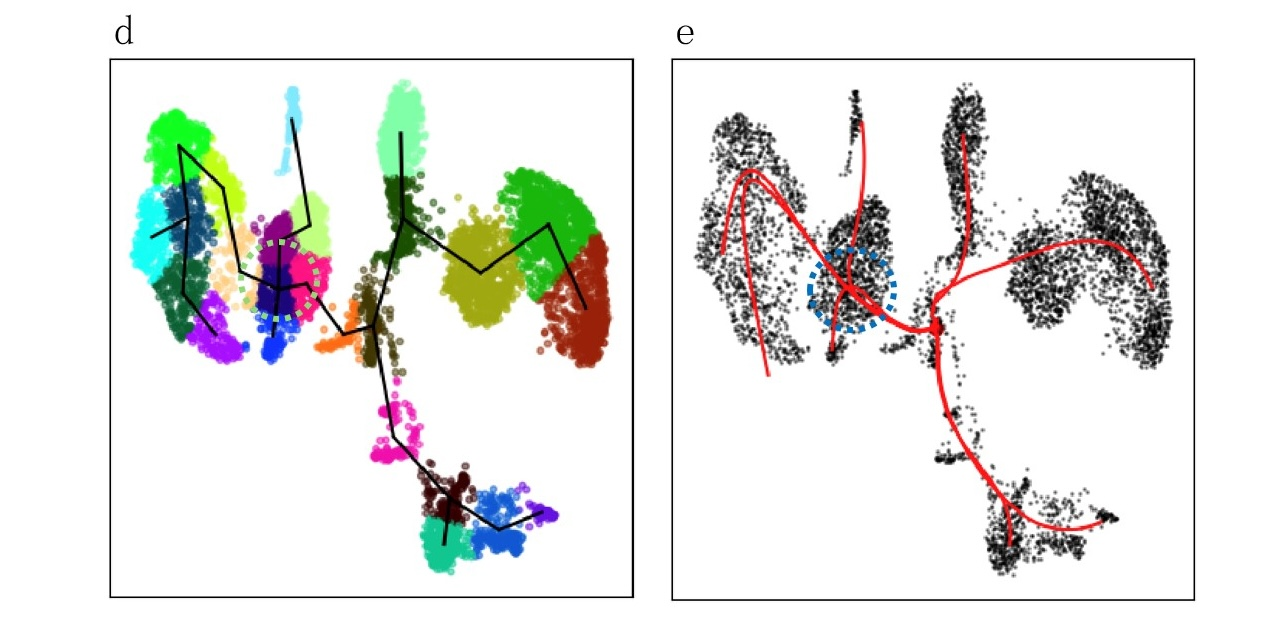
\includegraphics[width=\textwidth]{./img/Slide4.jpg}
    \end{center}
    \textbf{図2:} 解析結果の比較図
    \textbf{a} 制約付きの最小全域木
    \textbf{b} 制約付きの最小全域木を使用した解析結果
    \textbf{c} 制約無しの最小全域木
    \textbf{d} 制約無しの最小全域木を使用した解析結果
  \end{tcolorbox}
  \item Human fetal immune cells data
  ここに解析の方法や結果の解釈を書く
  \begin{tcolorbox}[colframe=black!70, colback=white, boxrule=0.2mm, width=\textwidth, arc=2mm]
    \begin{center}
        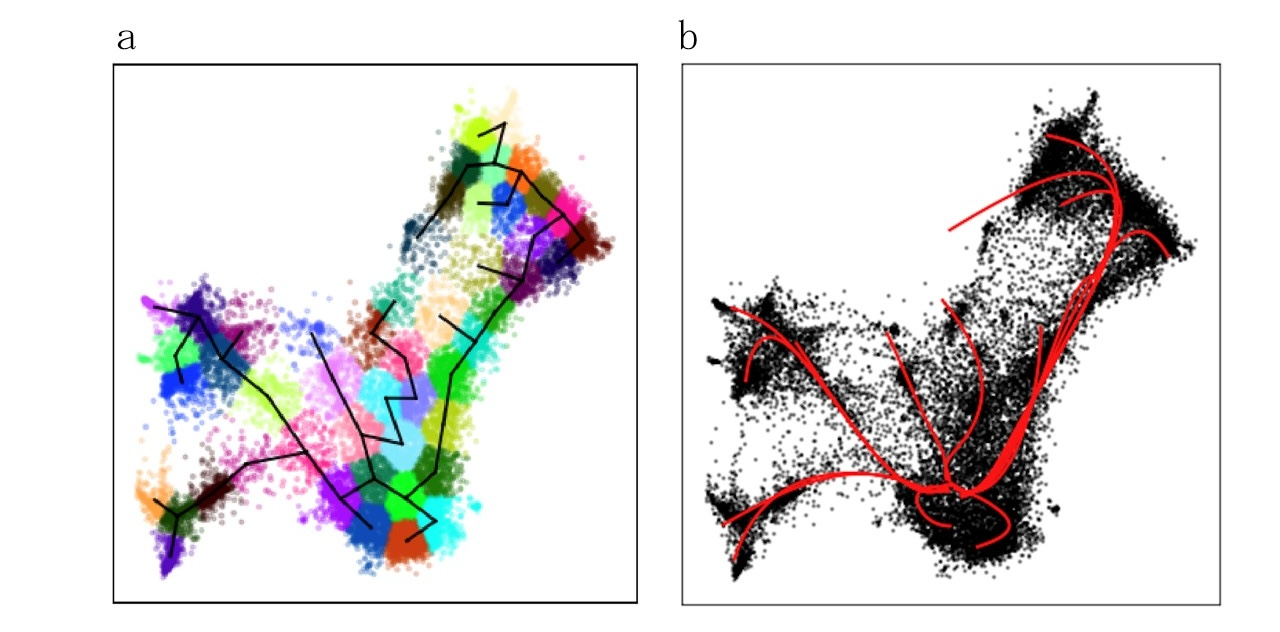
\includegraphics[width=\textwidth]{./img/Slide5.jpg}
        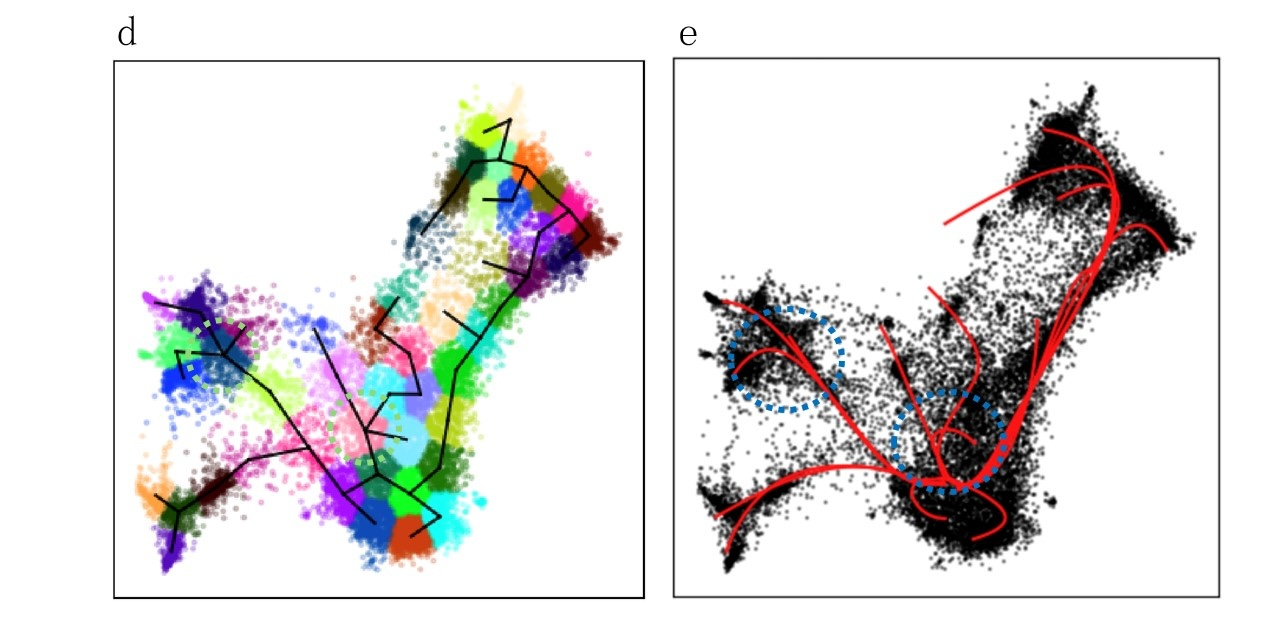
\includegraphics[width=\textwidth]{./img/Slide6.jpg}
    \end{center}
    \textbf{図3:} 解析結果の比較図
    \textbf{a} 制約付きの最小全域木
    \textbf{b} 制約付きの最小全域木を使用した解析結果
    \textbf{c} 制約無しの最小全域木
    \textbf{d} 制約無しの最小全域木を使用した解析結果
  \end{tcolorbox}
\end{itemize}


\subsection{堅牢性}\label{subsec-instruction-3}
ここに解析の方法や結果の解釈を書く
目的等
\begin{tcolorbox}[colframe=black!70, colback=white, boxrule=0.2mm, width=\textwidth, arc=2mm]
  \begin{center}
      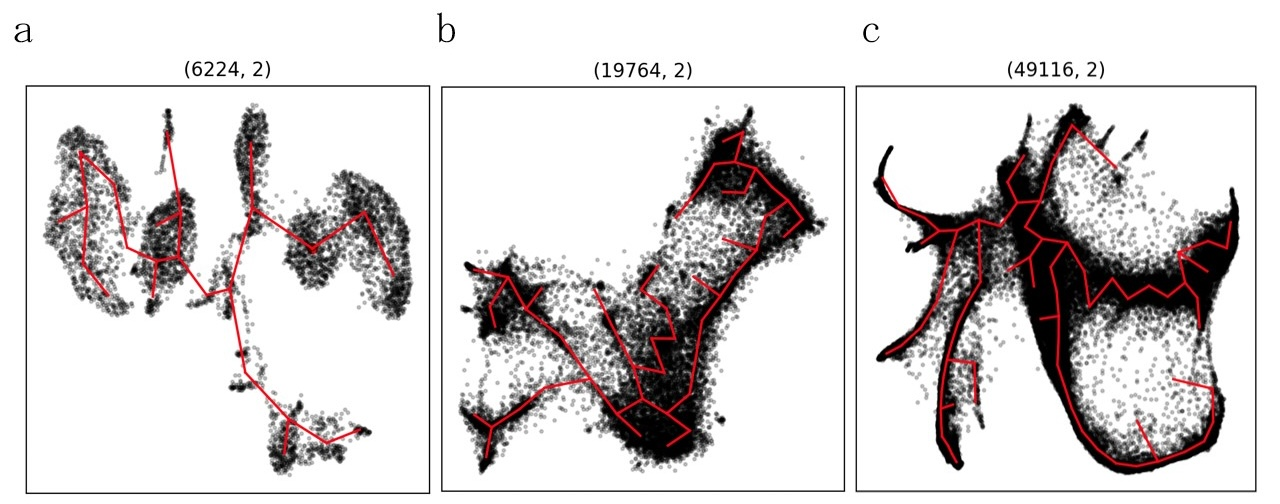
\includegraphics[width=\textwidth]{./img/Slide9.jpg}
      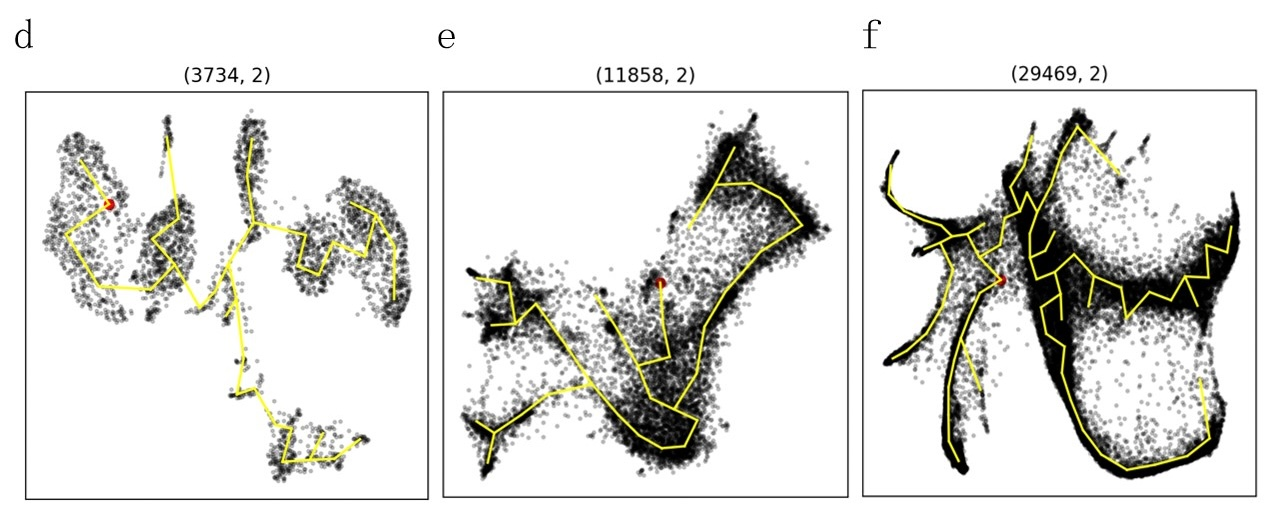
\includegraphics[width=\textwidth]{./img/Slide10.jpg}
  \end{center}
  \textbf{図4:} 解析結果の比較図
  \textbf{a} 制約付きの最小全域木
  \textbf{b} 制約付きの最小全域木を使用した解析結果
  \textbf{c} 制約無しの最小全域木
  \textbf{d} 制約無しの最小全域木を使用した解析結果
  \textbf{e} 制約無しの最小全域木を使用した解析結果
  \textbf{f} 制約無しの最小全域木を使用した解析結果
\end{tcolorbox}
\subsection{他のツールとの比較}\label{subsec-instruction-4}
\begin{tcolorbox}[colframe=black!70, colback=white, boxrule=0.2mm, width=\textwidth, arc=2mm]
  \begin{center}
      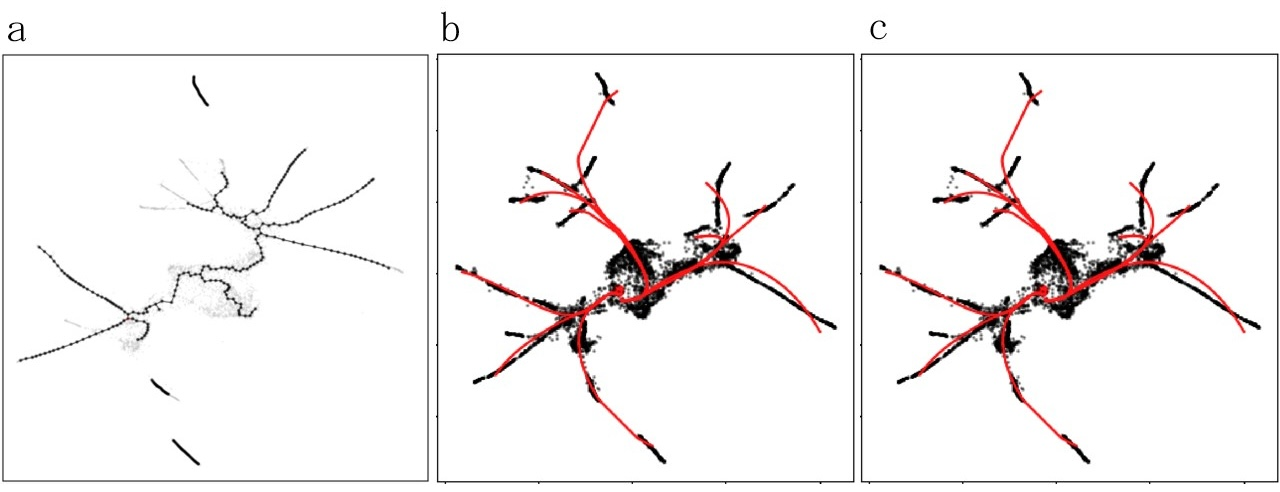
\includegraphics[width=\textwidth]{./img/Slide8.jpg}
  \end{center}
  \textbf{図5:} 解析結果の比較図
  \textbf{a} 制約付きの最小全域木
  \textbf{b} 制約付きの最小全域木を使用した解析結果
  \textbf{c} 制約無しの最小全域木
  \textbf{d} 制約無しの最小全域木を使用した解析結果
  \textbf{e} 制約無しの最小全域木を使用した解析結果
  \textbf{f} 制約無しの最小全域木を使用した解析結果
\end{tcolorbox}
\subsection{予測精度}\label{subsec-instruction-5}

  \begin{table}[h]
  \centering
  \begin{tabular}{|l|c|c|c|c|c|}
  \hline
  \textbf{状態} & \textbf{データ数} & \textbf{制約付正答数} & \textbf{制約付正答率} & \textbf{制約無正答数} & \textbf{制約無正答率} \\
  \hline
  Meg          & 1064 & 1064 & 1      & 0    & 0      \\
  Erythroid    & 365  & 365  & 1      & 0    & 0      \\
  Mast         & 1545 & 1545 & 1      & 1545 & 1      \\
  Baso         & 5998 & 5989 & 0.9985 & 5989 & 0.9985 \\
  Eos          & 168  & 0    & 0      & 0    & 0      \\
  Neutrophil   & 9231 & 9208 & 0.9975 & 9208 & 0.9975 \\
  Monocyte     & 9184 & 9069 & 0.9875 & 9069 & 0.3983 \\
  pDC          & 49   & 0    & 0      & 0    & 0      \\
  Lymphoid     & 64   & 0    & 0      & 0    & 0      \\
  Ccr7\_DC     & 203  & 0    & 0      & 0    & 0      \\
  \hline
  合計         & 27871 & 27240 & 0.5983 & 25811 & 0.4979 \\
  \hline
  \end{tabular}
  \caption{\textbf{表1:} Hematopoiesisに対する予測結果}
  \end{table}


\section{方法}\label{sec-structure}
\subsection{画像処理}\label{subsec-structure-1}
  \begin{itemize}
    \item 概要
    \item アルファシェイプ
    \item 細線化処理
    \item 重心点の計算
    \item 解像度とクラスタ数の関係
    \begin{table}[h]
      \centering
      \begin{minipage}[b]{0.49\columnwidth}
        \centering
        \scriptsize % ここでフォントサイズを小さくします
        \begin{tabular}{|c|c|c|c|}
        \hline
        \textbf{解像度} & \textbf{オブジェクト数} & \textbf{クラスタ数} & \textbf{面積} \\
        \hline
        10  & 1  & 4   & 0.9   \\
        20  & 8  & 8   & 0.245 \\
        30  & 3  & 15  & 0.919 \\
        40  & 3  & 30  & 0.826 \\
        50  & 11 & 25  & 0.269 \\
        60  & 17 & 51  & 0.237 \\
        70  & 9  & 60  & 0.283 \\
        80  & 16 & 82  & 0.247 \\
        90  & 44 & 128 & 0.173 \\
        \hline
        \end{tabular}
        \caption{\textbf{表2:} Bone marrow mononuclear cell}
      \end{minipage}
      \begin{minipage}[b]{0.49\columnwidth}
        \centering
        \scriptsize % ここでもフォントサイズを小さくします
        \begin{tabular}{|c|c|c|c|}
        \hline
        \textbf{解像度} & \textbf{オブジェクト数} & \textbf{クラスタ数} & \textbf{面積} \\
        \hline
        10  & 1  & 0   & 0.9   \\
        20  & 2  & 5   & 0.345 \\
        30  & 4  & 23  & 0.804 \\
        40  & 19 & 26  & 0.633 \\
        50  & 19 & 50  & 0.638 \\
        60  & 10 & 42  & 0.293 \\
        70  & 10 & 56  & 0.311 \\
        80  & 12 & 60  & 0.27  \\
        90  & 25 & 104 & 0.229 \\
        \hline
        \end{tabular}
        \caption{\textbf{表3:} Human fetal immune cells data}
      \end{minipage}
    \end{table}
    \begin{table}[h]
      \centering
      \begin{minipage}[b]{0.49\columnwidth}
        \centering
        \scriptsize % ここでフォントサイズを小さくします
        \begin{tabular}{|c|c|c|c|}
        \hline
        \textbf{解像度} & \textbf{オブジェクト数} & \textbf{クラスタ数} & \textbf{面積} \\
        \hline
        10  & 1  & 6   & 0.37  \\
        20  & 8  & 15  & 0.315 \\
        30  & 11 & 19  & 0.289 \\
        40  & 1  & 16  & 0.968 \\
        50  & 5  & 46  & 0.817 \\
        60  & 27 & 83  & 0.627 \\
        70  & 33 & 112 & 0.646 \\
        80  & 36 & 168 & 0.66  \\
        90  & 22 & 58  & 0.221 \\
        \hline
        \end{tabular}
        \caption{\textbf{表3:} Hematopoiesis}
      \end{minipage}
      \begin{minipage}[b]{0.49\columnwidth}
        \centering
        \scriptsize % ここでもフォントサイズを小さくします
        \begin{tabular}{|c|c|c|c|}
        \hline
        \textbf{解像度} & \textbf{オブジェクト数} & \textbf{クラスタ数} & \textbf{面積} \\
        \hline
        100  & 18   & 76    & 0.216 \\
        200  & 87   & 331   & 0.197 \\
        300  & 365  & 729   & 0.22  \\
        400  & 775  & 1242  & 0.161 \\
        500  & 1231 & 1544  & 0.129 \\
        600  & 2187 & 1959  & 0.062 \\
        700  & 2535 & 2465  & 0.062 \\
        800  & 3050 & 2603  & 0.048 \\
        900  & 3710 & 2774  & 0.036 \\
        \hline
        \end{tabular}
        \caption{\textbf{表4:} Hematopoiesis}
      \end{minipage}
    \end{table}
   

    \item クラスタ数と分岐認識能力
    \begin{tcolorbox}[colframe=black!70, colback=white, boxrule=0.2mm, width=\textwidth, arc=2mm]
      \begin{center}
          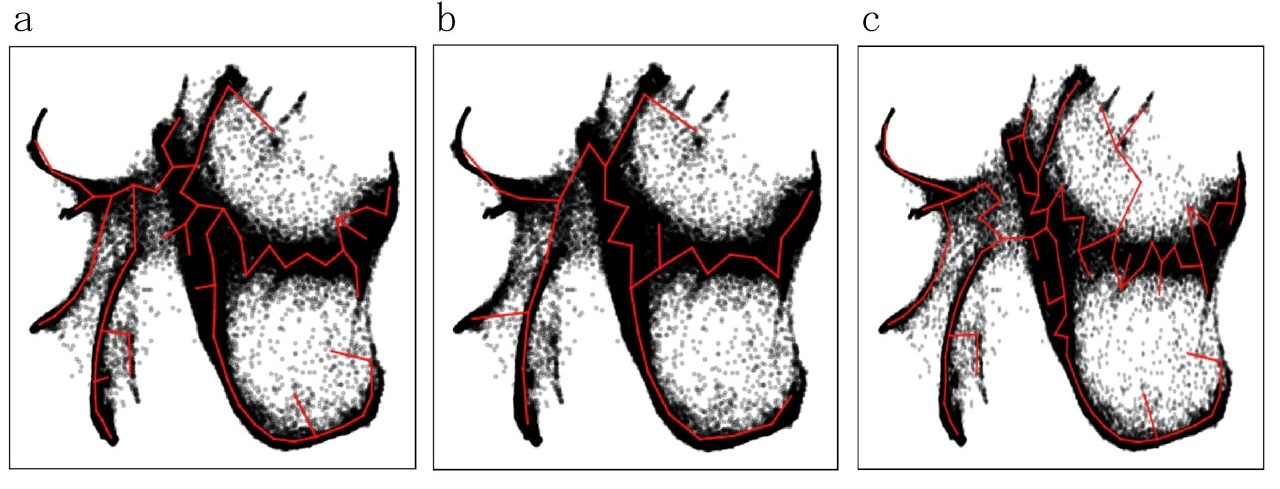
\includegraphics[width=\textwidth]{./img/Slide7.jpg}
      \end{center}
      \textbf{図6:} 解析結果の比較図
      \textbf{a} 制約付きの最小全域木
      \textbf{b} 制約付きの最小全域木を使用した解析結果
      \textbf{c} 制約無しの最小全域木
    \end{tcolorbox}
  \end{itemize}
\subsection{次数制約付き最小全域木}\label{subsec-abstract}

無向グラフ $G$
$G = (V, E)$

グラフ $G$ の頂点集合
$i, j \in V$

グラフ $G$ の辺集合
$(i, j) \in E, e \in E$

各辺 $e \in E$ の長さ
$d_e$


\[
\text{minimize} \quad \sum_{e \in E} d_e x_e
\]

\[
\text{s.t.} \quad
\begin{aligned}
    &\sum_{e \in E} x_e = |V| - 1, \\
    &\sum_{e \in \delta(\{i\})} x_e \leq 3 \quad \forall i \in V, \\
    &\sum_{i \in S} \sum_{j \in V \setminus S} x_{ij} \geq 1 \quad \forall S \subset V, \\
    &x_e \in \{0, 1\} \quad \forall e \in E.
\end{aligned}
\]

\end{document}
